\documentclass{article}
\usepackage{graphicx}
\usepackage{xcolor}
\usepackage{amsmath}
\usepackage[utf8]{inputenc}
\usepackage[T1]{fontenc}
\renewcommand{\rmdefault}{ptm}
\renewcommand{\sfdefault}{ptm}
\renewcommand{\ttdefault}{ptm}
\usepackage[french]{babel}
\usepackage{textcomp}
% Si vous voulez réinitialiser la numérotation des sections et pages à un certain point
\usepackage{titlesec}
\usepackage{url}
\usepackage{ragged2e}
\usepackage{enumitem}
\usepackage{float}
\usepackage[a4paper, margin=2.5cm]{geometry}  % Ajuster les marges à 2.5 cm de chaque côté
\renewcommand{\thesection}{\arabic{section}} % Utiliser des chiffres arabes pour la numérotation des sections

\begin{document}
% Page de couverture
\begin{titlepage}
    \centering
    
\includegraphics[width=0.4\textwidth]{ressources/logoSorbonne.png}
    \begin{center}
        \hrulefill \\[1cm]
        \Huge\textbf{Sorbonne Université} \\[1cm]
        \Large\textbf{Master 2 Science et Technologie du Logiciel} \\ [1cm]
        \hrulefill \\[1cm]
        \huge\textbf{Développement des Algorithmes d’Application Réticulaire} \\[1cm]
        \huge\textbf{\textcolor{cyan}{Projet final - Moteur de recherche d’une bibliothèque}} \\[2cm]
        \hrulefill \\[1.5cm]
        \Large\textbf{Auteurs:} Florian CODEBECQ, Nandraina RAZAFINDRAIBE\\[1cm] 
        \Large\textbf{Responsable:} Binh-Minh BUI-XUAN\\[2.5cm]
        \textbf{Année scolaire:} 2024/2025  
    \end{center}
\end{titlepage}

% Page suivant %
\newpage

\tableofcontents

\newpage

\setcounter{page}{1}

\setcounter{section}{0}
\section{Introduction}
Dans un monde où l’accès à l’information est primordial, les moteurs de recherche sont devenus des outils indispensables pour naviguer efficacement à travers les vastes collections de documents numériques. Ce projet s’inscrit dans cette problématique en proposant la conception et l’implémentation d’une application web et mobile dédiée à la recherche de documents textuels au sein d’une bibliothèque numérique.

Notre travail répond aux exigences du projet, qui vise à développer une application web et mobile permettant une recherche efficace de livres dans une bibliothèque numérique. Grâce à une base de données contenant plusieurs milliers d’ouvrages sous format textuel, l’objectif est de concevoir un moteur de recherche performant, capable de répondre aux requêtes des utilisateurs de manière pertinente et rapide.

L’approche adoptée repose sur l’exploitation d’algorithmes avancés pour l’indexation et le classement des résultats, en s’appuyant sur des concepts de centralité et de similarité. L’application ne se limite pas à une simple recherche par mots-clés, mais propose également des fonctionnalités avancées permettant une exploration plus fine du contenu textuel.

Au-delà de la conception technique, ce projet vise également à analyser la pertinence et la performance du moteur de recherche, en évaluant son comportement sur un grand volume de données. L’expérience utilisateur reste au cœur des préoccupations, avec une interface intuitive et une capacité à s’adapter aux besoins des lecteurs.
\section{Définition de problème et structures de données utilisées}
    \subsection{Définition du Problème de Recherche d'Information}
    Rechercher un livre dans une vaste collection nécessite un système capable d'extraire les documents pertinents en fonction de mots-clés spécifiques. Il s'agit de permettre à un utilisateur de retrouver des livres en fonction des mots ou expressions régulières qu'ils contiennent, dans une collection volumineuse où la recherche manuelle serait impraticable Au-delà de la simple recherche textuelle, le système classe les documents selon leur pertinence et propose des suggestions basées sur la similarité entre les livres. Cette approche assure une navigation fluide et une exploration efficace du contenu disponible.

    \subsection{Stockage et Indexation des Documents}
    Pour répondre efficacement à ces exigences, nous avons conçu une architecture de stockage à deux niveaux. Les documents textuels, téléchargés depuis \textbf{The Gutenberg Project}\cite{gutenberg}, sont conservés dans leur format original $(.txt)$ au sein d’un répertoire dédié, assurant ainsi leur intégrité. Leurs métadonnées sont parallèlement stockées au format JSON pour en faciliter l’exploitation et la représentation.

    Afin d’optimiser les performances de recherche, nous avons implémenté en Python une table d’indexation sous forme de dictionnaire de données (\textit{HashMap}). Chaque terme significatif y est associé à la liste des documents dans lesquels il apparaît, avec un score pondéré par TF-IDF. Cette structure clé permet d’accélérer les requêtes en évitant un parcours exhaustif des textes.
    \[
        \text{TF-IDF}(t, d) = \text{TF}(t, d) \times \text{IDF}(t)
    \]
    \[
        \text{TF}(t, d) = \frac{f_{t,d}}{\sum_{t' \in d} f_{t',d}}
    \]
    \[
        \text{IDF}(t) = \log \left( \frac{N}{|\{d \in D : t \in d\}|} \right)
    \]
    où :
    \begin{itemize}
        \item \( \text{TF}(t, d) \) (\textbf{Term Frequency}) : fréquence du terme $t$ dans le document $d$, normalisée par le nombre total de termes dans $d$.
        \item \( \text{IDF}(t) \) (\textbf{Inverse Document Frequency}) : mesure l’importance du terme $t$ en fonction de son apparition dans l’ensemble des documents $D$.
        \item  \( f_{t,d} \) : fréquence brute du terme $t$ dans le document $d$.
        \item $N$ : nombre total de documents.
        \item \( \left| \{d \in D : t \in d\} \right| \) : nombre de documents contenant le terme $t$.
    \end{itemize}
    
    Pour faciliter l’obtention des scores TF-IDF, Python offre la méthode TfidfVectorizer à travers sa bibliothèque scikit-learn\cite{scikitlearn}. La complexité globale de cette méthode est estimée comme ~ $O(n*m)$ sur un corpus de $n$ documents contenant un total de $m$ mots avec des optimisations internes utilisées par scikit-learn. 
    
    Quant à la construction de la table d’index, nous avons pris en entrée le résultat de la méthode TfidfVectorizer. Ensuite, en $O(T \times N)$ où avec $T$ étant le nombre de termes et $N$ étant le nombre de livres, nous obtenons la table d’index dans laquelle chaque terme est associé aux livres qui le concernent\cite{coursrechercheinfo}.

    \subsection{Graphes de Jaccard et similarité documentaire}
    Pour mettre en œuvre les fonctionnalités de suggestion, nous avons construit un graphe de Jaccard représenté par une matrice d'adjacence. Chaque livre est représenté comme un nœud dans un graphe. Cette structure modélise les relations de similarité entre les documents, chaque arête étant pondérée selon la distance de Jaccard calculée entre deux livres. La liaison entre 2 nœuds est établie si la distance entre ces 2 nœuds est inférieure à un seuil (0.5 dans notre cas). Cette mesure, basée sur le rapport entre l'intersection et l'union des ensembles de termes contenus dans les documents, permet d'identifier des textes thématiquement proches même lorsqu'ils ne partagent pas exactement les mêmes mots-clés recherchés par l'utilisateur. 

    La computation d’un tel algorithme s’exécute en $O(N^2 \times (k_1 + k_2))$ où le nombre total de paires de livres est $\frac{N \times (N-1)}{2}$, soit $O(N^2)$.  $k_1$ et $k_2$ sont respectivement les tailles des ensembles de mots-clés pour les livres pris deux à deux.
    Ce modèle permet non seulement d’améliorer la classification des résultats de recherche, mais aussi d’offrir des recommandations pertinentes aux utilisateurs.

    \subsection{Indices de centralité et classement des résultats}
    Le classement pertinent des résultats constitue un aspect essentiel de notre moteur de recherche. Pour dépasser le simple comptage d'occurrences, nous avons implémenté des indices de centralité attribués à chaque document dans le graphe de Jaccard. Ces indices, calculés selon des algorithmes de théorie des graphes, permettent d'évaluer l'importance relative de chaque livre au sein de l'ensemble de la bibliothèque. Un document possédant une forte centralité sera considéré comme plus représentatif ou influent, et se verra donc attribuer un rang supérieur dans les résultats de recherche. 

    Pour la pondération des résultats, on a utilisé cette règle suivante : 
    \begin{quote}
        Pour chaque document $d_i$ dans les résultats, le score de pertinence est calculé comme suit
        \[
            P(d_i) = \textit{tfidf}_i \times \left( c_i + \epsilon \right)
        \]
        Où :
        \begin{itemize}
            \item \( \textit{tfidf}_i \) est le score TF-IDF du document \( d_i \).
            \item \( c_i \) est le score de centralité du document \( d_i \).
            \item \( \epsilon \) est un petit biais ajouté pour éviter que les documents sans score de centralité aient un score nul.
        \end{itemize}
    \end{quote}

    Les résultats sont ensuite triés par ordre décroissant de leur score de pertinence.
    Les indices de centralité, tels que le betweenness, le closeness et le PageRank, sont déjà implémentés dans la bibliothèque  \textit{NetworkX}\cite{networkx} de Python. La matrice d’adjacence, la table d’index ainsi que les indices de centralité sont stockés dans un objet sérialisé Python afin de faciliter l’accès aux données lors de la recherche.

    L’utilisateur pourra spécifier l’indice de centralité de son choix pour le classement dans la recherche avancée. Nous détaillerons davantage ces mesures de centralité dans la section suivante.

\section{Présentation théorique des algorithmes}
    \subsection{Algorithme de Knuth-Morris-Pratt (KMP)}
    L’algorithme de Knuth-Morris-Pratt (KMP) est utilisé pour rechercher un motif dans un texte en temps linéaire. Contrairement à l'approche naïve, KMP évite les comparaisons redondantes en utilisant les informations des correspondances partielles déjà établies.

    \textbf{Fonctionnement} :
    \begin{itemize}
        \item \textit{Prétraitement} : KMP commence par prétraiter le motif \( F \) pour générer un tableau de préfixes qui est aussi de suffixe ou LPS (Longest Proper Prefix). Cette table contient l’information sur les préfixes et suffixes qui se répètent dans le motif. La longueur de cette table est la même que celle du motif. On peut obtenir le LPS en utilisant cet algorithme : 
            
        Pour tout \( i \), nous avons :
            \begin{align}
                \text{LPS}[i] &= \text{taille du plus long préfixe-suffixe de } F[0 \dots i-1] \\
                \text{Si } F[i] &= F[\text{LPS}[i]] \quad \text{alors} \quad \text{LPS}[i] = \text{LPS}[\text{LPS}[i]]
            \end{align}
        (2) correspond à une optimisation de LPS.
        \item \textit{Recherche} : Lors de la recherche dans le texte, si une erreur de correspondance se produit, l’algorithme utilise la table pour sauter les comparaisons inutiles, ce qui permet d’éviter de revenir en arrière dans le texte.
    \end{itemize}

    \textbf{Comparaison avec d’autres algorithmes} :
    \begin{itemize}
        \item \textit{Naïve} : L’algorithme naïf compare chaque caractère du motif avec chaque caractère du texte, ce qui donne une complexité de $O(T \times M)$. L’algorithme KMP améliore cette complexité en $O(T + M)$.
        \item \textit{Boyer-Moore} : Le Boyer-Moore \cite{lecroq1992variation} est généralement plus rapide que KMP, surtout pour les textes longs, en exploitant des heuristiques de saut basées sur les caractères du motif. Cependant, KMP peut être plus rapide sur des motifs courts ou des textes avec peu de répétitions.
    \end{itemize}   
    
    \subsection{Algorithme d’Aho-Ullman}
    L’algorithme Aho-Ullman est une méthode efficace pour effectuer une recherche simultanée de plusieurs motifs dans un texte. Cette approche consiste à construire un automate fini à partir d’une expression régulière. Cet algorithme d’Aho-Ullman \cite[Chapter~10]{aho1992foundations} comporte  plusieurs étapes :
    \begin{itemize}
        \item \textit{Construction d’un arbre syntaxique à partir d’une expression régulière.}  
        Cette étape consiste à transformer l'expression régulière en un arbre syntaxique qui représente sa structure logique. Cet arbre décompose l'expression en opérateurs (concaténation, union, fermeture de Kleene) et opérandes (symboles de l'alphabet).
        \item \textit{Conversion de cet arbre en un automate fini non déterministe (AFND) avec $\epsilon$-transition.}
        L’automate fini non déterministe avec $\epsilon$-transitions (\textit{AFND}-$\epsilon$) est construit en appliquant les algorithmes de Thompson :
        Chaque feuille de l’arbre syntaxique est un état avec une transition associée. Les nœuds internes appliquent les règles de concaténation, union et étoile de Kleene\cite{kleene1951representationof}. Des transitions $\epsilon$ sont utilisées pour relier les états intermédiaires, facilitant ainsi la construction.
        \begin{figure}[h] % Utilisation de l'option [h] pour placer l'image ici
            \centering
            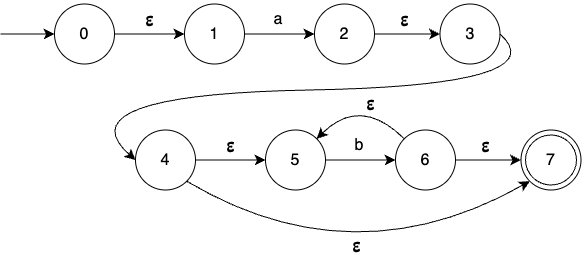
\includegraphics[width=0.75\textwidth]{./ressources/NDFA.drawio.png}
            \caption{Représentation \textit{AFND} de a.b*}
            \cite{schemaAutomate}
            \label{fig:schemaAutomateNDFA}
        \end{figure}
        \item \textit{Transformer de l’automate fini non déterministe en un automate fini déterministe (\textit{AFD}).}
        L’automate fini déterministe (\textit{AFD}) est obtenu en éliminant les transitions $\epsilon$ via l’algorithme de déterminisation par construction des sous-ensembles (Subset Construction) :
        \begin{itemize}
            \item Chaque état de l’\textit{AFD} correspond à un ensemble d’états de l’\textit{AFND}.
            \item On fusionne les transitions possibles pour chaque symbole afin de garantir l’unicité du prochain état.
        \end{itemize}
        \begin{figure}[H] % Utilisation de l'option [h] pour placer l'image ici
            \centering
            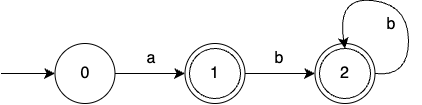
\includegraphics[width=0.5\textwidth]{./ressources/DFA.drawio.png}
            \caption{Représentation \textit{AFD} de a.b*}
            \cite{schemaAutomate}
            \label{fig:schemaAutomateDFA}
        \end{figure}
        \item \textit{Optimiser l’\textit{AFD} afin d’obtenir un automate avec un nombre minimum d’états.}
        L’\textit{AFD} peut être réduit pour minimiser le nombre d’états, en appliquant l’algorithme de minimisation de Hopcroft : 
        \begin{itemize}
            \item On regroupe les états équivalents en classes d’équivalence.
            \item On élimine les états inutiles et fusionne ceux ayant le même comportement.
        \end{itemize}
        L’automate résultant est minimal, garantissant un coût de reconnaissance optimal.
        \begin{figure}[H] % Utilisation de l'option [h] pour placer l'image ici
            \centering
            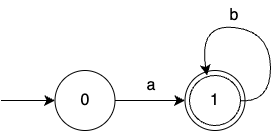
\includegraphics[width=0.35\textwidth]{./ressources/DFA_optimized.drawio.png}
            \caption{Représentation \textit{AFD optimisé} de a.b*}
            \cite{schemaAutomate}
            \label{fig:schemaAutomateDFAOptimized}
        \end{figure}
    \end{itemize}

    \subsection{ Mesure de Similarité de Jaccard}
    La mesure de similarité de Jaccard est utilisée pour comparer deux ensembles et déterminer leur degré de ressemblance. Elle est particulièrement utilisée dans l’analyse de texte, la classification de documents, et la détection de similarité entre corpus textuels ou ensembles de données.	
    
    Soient \( A \) et \( B \) deux ensembles représentant respectivement les termes présents dans les documents \( D_A \) et \( D_B \).

    $J(A, B)$ est la similarité de Jaccard, donnée par la formule :
    \[
    J(A, B) = \frac{|A \cap B|}{|A \cup B|}
    \]

    La distance de Jaccard est donc :
    \[
    d_J(A, B) = 1 - J(A, B)
    \]

    Cette distance varie entre 0 et 1. Lorsque \( d_J(A, B) = 0 \), les ensembles sont identiques. À l'inverse, si \( d_J(A, B) = 1 \), cela signifie que les ensembles sont totalement différents et n'ont aucune intersection.

    Il en existe d’autres mesures de similarité comme \textit{Cosinus} et \textit{Dice}. La similarité cosinus est utilisée pour mesurer la proximité angulaire entre deux vecteurs représentant des documents. Contrairement à Jaccard, elle prend en compte les fréquences des termes. Elle est adaptée aux documents longs avec pondération TF-IDF mais ne distingue pas les mots rares des mots fréquents.
    
    Soient \( A \) et \( B \) deux vecteurs représentant des documents dans un espace de dimension \( n \), où chaque dimension correspond à un terme du vocabulaire. Les composantes de ces vecteurs sont les scores TF-IDF des termes présents dans les documents.

    La similarité cosinus entre ces deux documents est donnée par :
    \[
    \cos(A, B) = \frac{\sum_{i=1}^{n} A_i B_i}{\sqrt{\sum_{i=1}^{n} A_i^2} \times \sqrt{\sum_{i=1}^{n} B_i^2}}
    \]

    où \( A = (A_1, A_2, \dots, A_n) \) et \( B = (B_1, B_2, \dots, B_n) \) sont les vecteurs TF-IDF des documents.

    La similarité de Dice est une variante de Jaccard avec un poids supplémentaire sur les éléments communs. Dice est plus sensible aux petits ensembles mais moins interprétable que Jaccard sur de grands corpus.
    
    Soient \( A \) et \( B \) deux ensembles représentant respectivement les termes présents dans les documents \( D_A \) et \( D_B \).
    
    La similarité de Dice entre ces deux documents est donnée par :
    \[
        D(A, B) = \frac{2 |A \cap B|}{|A| + |B|}
    \]

    Lee (1999)\cite{lee2000measures}  dans "Measures of distributional similarity" a démontré que "la similarité cosinus offre généralement de meilleurs résultats pour les comparaisons de textes complets, tandis que Jaccard est plus adapté pour les représentations par ensembles de mots-clés ou de caractéristiques discrètes."

    \subsection{ Closeness Centrality }
    La centralité de proximité (\textit{Closeness Centrality}) est une mesure qui quantifie la proximité d'un nœud par rapport à tous les autres nœuds dans un graphe. Dans le contexte de notre bibliothèque numérique, elle permet d'identifier les documents qui sont "proches" de nombreux autres documents en termes de contenu, suggérant ainsi leur caractère représentatif ou central dans la collection.
    \[
        C_C(v) = \frac{n - 1}{\sum_{u \neq v} d(v, u)}
    \]
    où :
    \begin{itemize}
        \item $n$ est le nombre total de nœuds dans le graphe,
        \item $d(v, u)$ est la distance la plus courte entre le nœud $v$ et un autre nœud $u$.
    \end{itemize}
    Plus $C_C(v)$ est grand, plus le nœud $v$ est “central” dans le graphe, car il est proche des autres nœuds en termes de distance. Comme l'expliquent Wasserman et Faust dans "Social Network Analysis: Methods and Applications" (1994)\cite{wasserman1994social}, les nœuds avec une forte centralité de proximité peuvent diffuser efficacement l'information à travers le réseau. Cela peut être utile dans des systèmes de recommandation de bibliothèques, où l’on cherche à mettre en avant les documents les plus “reliés” à d’autres.

    \subsection{ Betweenness Centrality }
    La centralité d'intermédiarité (\textit{Betweenness Centrality}) mesure la fréquence à laquelle un nœud se trouve sur les plus courts chemins entre d'autres nœuds du graphe. Un nœud avec une centralité de betweenness élevée agit comme un “pont” entre différents sous-graphes et joue un rôle crucial dans la connectivité globale du réseau.
    \[
        C_B(v) = \sum_{s \neq v \neq t} \frac{\sigma_{st}(v)}{\sigma_{st}}
    \]
    où :
    \begin{itemize}
        \item $\sigma_{st}(v)$ est le nombre de ces chemins qui passent par le nœud $v$.
        \item $\sigma_{st}$ est le nombre total de plus courts chemins entre les nœuds $s$ et  $t$,
    \end{itemize}
    Freeman (1977)\cite{freeman1977set}, dans son article fondateur "A Set of Measures of Centrality Based on Betweenness", explique que "les nœuds à forte intermédiarité contrôlent le flux d'information entre différentes parties du réseau."  Cette propriété est particulièrement utile dans notre moteur de recherche pour identifier les ouvrages interdisciplinaires ou ceux qui établissent des liens entre des domaines distincts.

    \subsection{ PageRank Centrality }
    Développé initialement par Brin et Page pour le moteur de recherche Google\cite{brin1998anatomy}, \textit{PageRank} est un algorithme qui attribue une pondération numérique à chaque élément d'un ensemble de documents liés par des hyperliens, dans le but de mesurer son importance relative au sein de cet ensemble. Dans notre adaptation, nous considérons les liens de similarité entre documents comme des "votes" d'importance, similaires aux hyperliens sur le web.

    Le score PageRank $PR(A)$ d'un document $A$ est calculé de manière itérative par :
    \[
        PR(A) = (1 - d) + d \times \sum_{i \in In(A)} \frac{PR(i)}{L(i)}
    \]
    où $PR(A)$ est le PageRank de la page $A$, $In(A)$ est l’ensemble des pages pointant vers $A, L(i)$ est le nombre de liens sortants de la page $i$, et d est un facteur d’amortissement (souvent pris égal à 0.85).

    Il existe aussi un autre indice, \textit{HITS (Hyperlink-Induced Topic Search)}, qui constitue une approche complémentaire. Contrairement aux autres mesures qui attribuent un score unique de centralité, \textit{HITS} distingue deux rôles distincts au sein du réseau :
    Le score d’autorité, qui évalue la pertinence d’un document en fonction du nombre et de la qualité des liens pointant vers lui.
    Le score de hub, qui mesure la capacité d’un document à orienter vers des ressources pertinentes.
    Cette distinction permet d’identifier à la fois les documents de référence riches en contenu (autorités) et ceux qui jouent un rôle d’aiguillage vers des informations importantes (hubs). Toutefois, cette sophistication implique une complexité de calcul plus élevée et une stabilité moindre par rapport aux approches comme \textit{PageRank}.

\newpage
\section{Conclusion}

\newpage
\bibliographystyle{unsrt}
\bibliography{references}
\end{document}